\section{Motivation} \label{intro}
There is not much work done around this topic and after reading the concepts
of network science it looks very interesting to find out how different module relate and how
these relations can be interpreted. This paper \textit{Power Laws in Software} \cite{louridas2008power} 
does analysis of power law distribution in a software application at class level and function level.
It did analysis of java, perl, c/c++ etc applications and did establish a pattern that 
these applications do follow power law distribution.

\begin{figure}[htbp]
\centering
\fbox{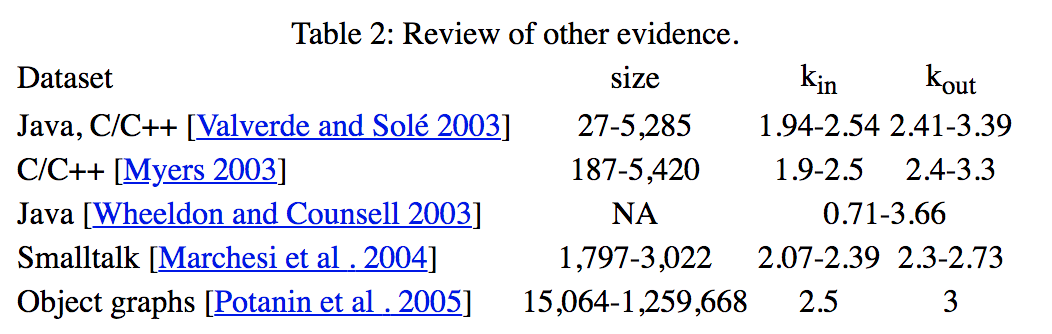
\includegraphics[width=\linewidth]{images/louridas2008power}}
\caption{Review of Languages}
\label{fig:louridas2008power}
\end{figure}

It depicts the size of datasets studied for this this analysis. However,
we couldn't find a paper or research which analyzes these patterns
 on all modules present in a given language.
Its very interesting problem to solve and find out how various python 
packages are dependent on each other and does it make sense 
to bundle some of the very common packages used along with base 
python distribution. It is interesting to understand the dependency structure 
but also to understand the community structure of these modules and 
what kind of network they form. Any other phenomenon exist when 
we analyze this graph. This analysis can be used to optimize the 
imports, remove cyclic dependencies between modules. Similar 
approach can be extended to other programming languages like java, ruby, perl etc.  